\documentclass{article}
\usepackage{graphicx}
\usepackage{hyperref}
\usepackage{listings}
\usepackage{xcolor}
\usepackage{tikzsymbols}
\usepackage{float}

\lstset{
    basicstyle=\ttfamily,
    backgroundcolor=\color{gray!30},
}

\title{Certificate Authority}
\begin{document}
\maketitle

\graphicspath{ {./Images/} }
\tableofcontents

\section{Introduction}
This explains how to configure the CA and sign certificates with it.
"The Enterprise CA offers features like Certificate Templates, Certificate Auto enrollment and Key archival. 
Enterprise CA is trusted by all domain joined clients."

\section{Prerequisites}
\begin {enumerate}
\item You should have joined the CA to the Domain.
\item You should be logged in as a \textbf{domain} administrator in the Cert Publishers group
\end {enumerate}

To add the Cert Publishers permission, RDP into one of the Domain Controllers.
Then add a user (probably the administrator) to the Cert Publishers group.

\begin{figure}[H]
        \centering
        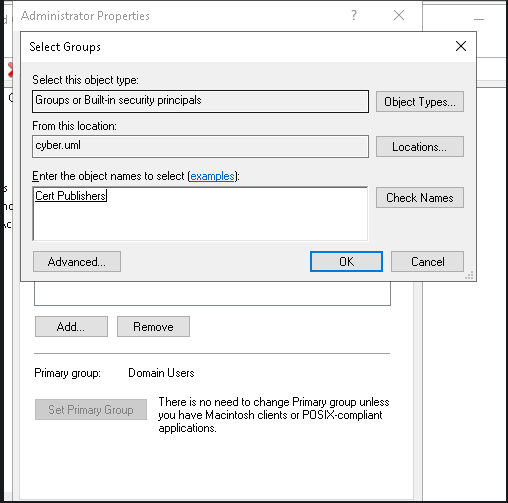
\includegraphics[width=1\textwidth]{AddingCertPublisherPermission.png}
        \caption{Adding administrator to the Cert Publishers group}
        \label{fig:AddingCertPublisherPermission}
\end{figure}

\begin{figure}[H]
        \centering
        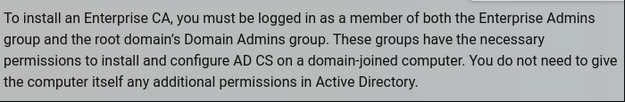
\includegraphics[width=1\textwidth]{BingOnPermissions.png}
        \caption{Bing on Permissions}
        \label{fig:BingOnPermissions}
\end{figure}

After adding the permission, you will need to log in and out of the CA for it to take effect.
Note that the domain administrator is possibly logged into differently than the local administrator.

Make sure to login with the administrator account, as seen in \ref{fig:ExampleLoginNETBIOS}

\begin{figure}[H]
        \centering
        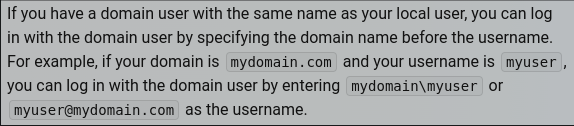
\includegraphics[width=1\textwidth]{BingDomainUserAdminUser.png}
        \caption{How to avoid possible naming conflicts}
        \label{fig:BingDomainUserAdminUser}
\end{figure}

\begin{figure}[H]
        \centering
        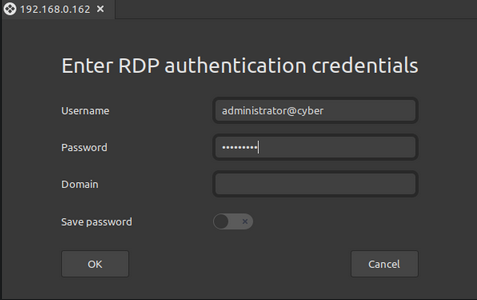
\includegraphics[width=1\textwidth]{ExampleLoginNETBIOS.png}
        \caption{Example login, explicitly with the Domain Administrator (note the @cyber to show it the domain admin, not the local admin)}
        \label{fig:ExampleLoginNETBIOS}
\end{figure}

Your domain admin account should now have the necessary permissions to configure the CA.

\section{Installing/Configuring Active Directory Certificate Services}

\begin{figure}[H]
        \centering
        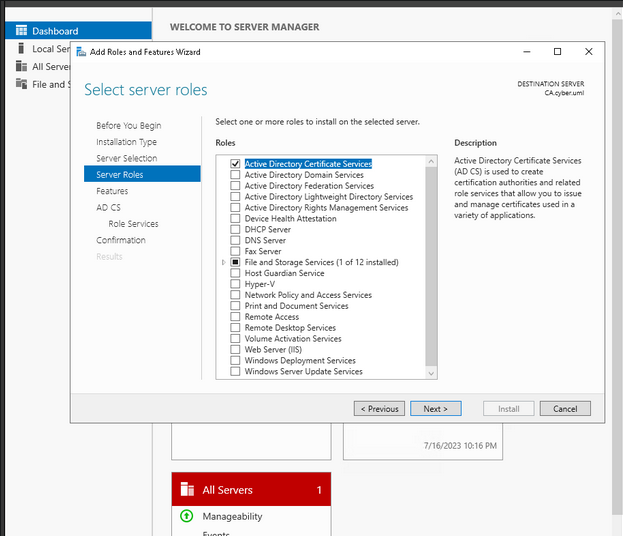
\includegraphics[width=1\textwidth]{ServerManager.png}
        \caption{Clicking the ADCS button}
        \label{fig:ADCS}
\end{figure}

Install Active Directory Certificate Services.


\begin{figure}[H]
        \centering
        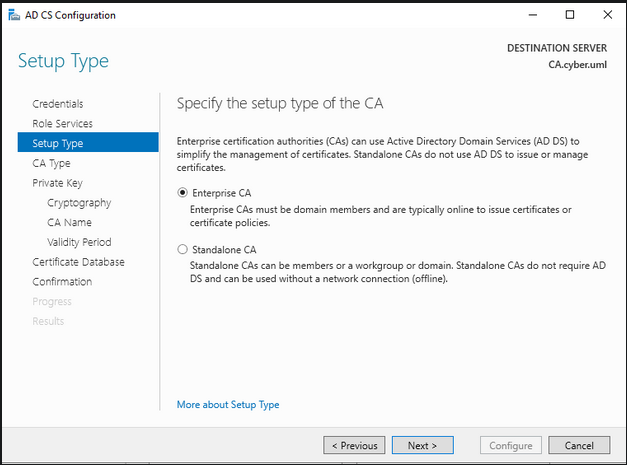
\includegraphics[width=1\textwidth]{EnterpriseCA.png}
        \caption{The only important button is the Enterprise CA button. Click it!}
        \label{fig:EnterpriseCA}
\end{figure}

Make sure to select Enterprise CA.

\begin{figure}[H]
        \centering
        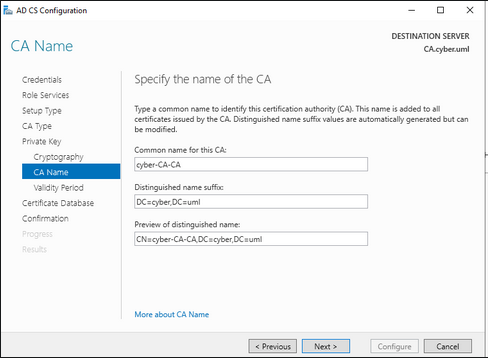
\includegraphics[width=1\textwidth]{CAName.png}
        \caption{Selecting the CA name}
        \label{fig:CAName}
\end{figure}

As long as it is unique it should be fine, to be safe we can probably stick with the hostname of the CA machine.

\subsection{Confirming the CA works}

To check the CA we need to make a certificate signing request. 
Unless you have someone who needs a cert, you can make a request by putting this in a text file called "example.inf"

\begin{lstlisting}[breaklines=true, columns=fullflexible]
[Version]
Signature="$Windows NT$"

[NewRequest]
Subject = "CN=example.com"
KeySpec = 1
KeyLength = 2048
Exportable = TRUE
MachineKeySet = TRUE
SMIME = False
PrivateKeyArchive = FALSE
UserProtected = FALSE
UseExistingKeySet = FALSE
ProviderName = "Microsoft RSA SChannel Cryptographic Provider"
ProviderType = 12
RequestType = PKCS10
KeyUsage = 0xa0

[RequestAttributes]
CertificateTemplate = WebServer

[EnhancedKeyUsageExtension]
OID=1.3.6.1.5.5.7.3.1 ; Server Authentication
\end{lstlisting}

\begin{figure}[H]
        \centering
        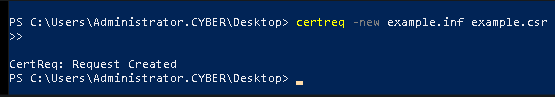
\includegraphics[width=1\textwidth]{MakingATestCertReq.png}
        \caption{Making a test certificate request}
        \label{fig:MakingATestCertReq}
\end{figure}

Open a PowerShell prompt, navigate to the directory where you saved the example.inf file, 
and run the following command
\begin{lstlisting}[breaklines=true, columns=fullflexible]
certreq -new example.inf example.csr
\end{lstlisting}

\begin{figure}[H]
        \centering
        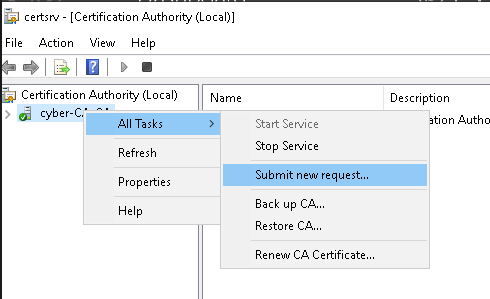
\includegraphics[width=1\textwidth]{SubmitNewRequest.png}
        \caption{Submitting the request to the CA}
        \label{fig:SubmitNewRequest}
\end{figure}

Open up certsrv, either by searching for "Certificate Authority" on the machine,
or by doing meta + r to run certsrv.msc. Right click on the CA's name (as in the screenshot),
hover over "All Tasks", and click "Submit New Request."

This prompts you to select the .csr file to submit.

\begin{figure}[H]
        \centering
        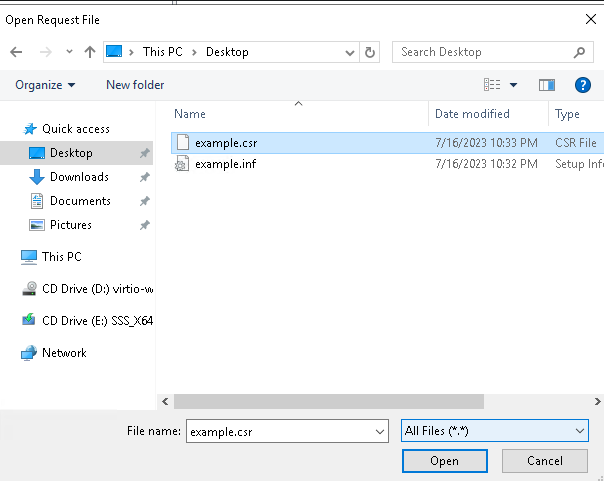
\includegraphics[width=1\textwidth]{SelectAllFiles.png}
        \caption{Select the .csr file. To find it, make sure to select "Show All Files" (on the bottom right)}
        \label{fig:ShowAllFiles}
\end{figure}

To approve the request, expand the menu. Then click "Pending Requests." Then approve the request.
\end{document}

